\documentclass[12pt]{article}



%%% RECOMMENDED
% better accented letters and ligatures in PDF
\usepackage[T1]{fontenc}
% set language of outputs (due to issues with TeX Live >= 2025 and LaTeXML <= 0.8.8, put 'british' in the *class* options!)
\usepackage{babel}
% PDF hyperlinks and metadata
\usepackage{hyperref}
\usepackage{xcolor}
\usepackage{setspace}
\definecolor{solframecol}{RGB}{32, 116, 44}
\definecolor{excol}{RGB}{235, 255, 235}
\definecolor{loframecol}{RGB}{0, 59, 176}
\definecolor{defcol}{RGB}{230, 230, 230}

\hypersetup{
    colorlinks=true,
    linkcolor=loframecol,
    filecolor=loframecol,      
    urlcolor=loframecol
    }
% higher quality variant of Computer Modern
\usepackage{lmodern}
% title and author
\usepackage{graphicx} % Required for inserting images
\usepackage[margin=1in]{geometry}
\usepackage{tikz,lipsum,lmodern}
\usepackage{amssymb}
\usepackage{amsmath}
\usepackage{amsthm}
\usepackage{enumerate}
\usepackage{bookml/bookml}
\usepackage{comment}
\usepackage{framed} 

\setlength{\parindent}{0pt}
\numberwithin{equation}{subsection}

\newtheorem{defn}{Definition}[subsection]
\theoremstyle{definition} 
\newtheorem{ex}{Example}[subsection]

\ifcsname insertBlanks\endcsname
    \iflatexml
        \newcommand{\blank}[1]{\<span style="display: inline-block; border-bottom: 1px solid black;">\<span style="visibility: hidden">{#1}{#1}\</span>\</span>}
    \else
      \newlength{\myl}
      \newcommand{\blank}[1]{\settowidth{\myl}{#1}
      \underline{\hspace{2\myl}}}
    \fi
\else
  \newcommand{\blank}[1]{#1}
\fi

\iflatexml % for the HTML
    \newenvironment{solution}{
        \<details>\<summary>Solution\</summary>\<div class="box-content">}
        {\</div>\</details>}
\else      % for the PDF
    \newenvironment{solution}{
    \bgroup\colorlet{TFFrameColor}{solframecol}\colorlet{TFTitleColor}{white}\begin{titled-frame}{Solution}}{\end{titled-frame}\egroup} 
\fi

%box for learning outcomes
\iflatexml % for the HTML
    \newenvironment{learningoutcomes}{
        \<div class="lo-box">
            \<div class="lo-box-title"> Learning Outcomes\</div>\<div class="box-content">}{\</div>\</div>}
\else      % for the PDF
    \newenvironment{learningoutcomes}{
    \bgroup\colorlet{TFFrameColor}{loframecol}\colorlet{TFTitleColor}{white}\begin{titled-frame}{Learning Outcomes}}{\end{titled-frame}\egroup} 
\fi


%box for examples
\iflatexml % for the HTML
    \newenvironment{example}{
            \<div class="ex-box"> \begin{ex}}        
            {\end{ex} \</div>}
\else      % for the PDF
    \newsavebox{\exbox}
    \newenvironment{example}
      {\begin{lrbox}{\exbox}%
       \begin{minipage}{\dimexpr\columnwidth-2\fboxsep\relax}
       \setlength{\parindent}{0pt}
       \begin{ex}}
      {\end{ex}\end{minipage}\end{lrbox}%
       \begin{center}
       \setlength{\fboxsep}{8pt}
       \colorbox{excol}{\usebox{\exbox}}
       \end{center}}
\fi


%box for definitions
\iflatexml % for the HTML
    \newenvironment{definition}{
            \<div class="def-box"> \begin{defn}}        
            {\end{defn} \</div>}
\else      % for the PDF
    \newsavebox{\defbox}
    \newenvironment{definition}
      {\begin{lrbox}{\defbox}%
       \begin{minipage}{\dimexpr\columnwidth-2\fboxsep\relax}
       \setlength{\parindent}{0pt}
       \begin{defn}}
      {\end{defn}\end{minipage}\end{lrbox}%
       \begin{center}
       \setlength{\fboxsep}{8pt}
       \colorbox{defcol}{\usebox{\defbox}}
       \end{center}}
\fi

\title{MATH19641: Mathematics 1Q1 \\Lecture Notes}
\author{Carl A. Whitfield}
\date{Semester 1 -- Academic Year 2026/27}

\onehalfspacing

\begin{document}

\setcounter{section}{-1}

\maketitle
\tableofcontents

\section{Introduction}

Welcome to the course notes for Mathematics 1Q1! For a general introduction to the course, including details of assessments, please visit the Course Unit Information module on Canvas. 

\subsection{Help and support}

\textbf{Me:} Carl Whitfield (you can call me Carl).\par
E-mail: \href{mailto:carl.whitfield@manchester.ac.uk} (Start with ``Hi Carl''). \par
Office hour: Mondays 10am-11am, Room 1.214 Alan Turing Building

\bigskip
\textbf{Piazza:} Ask questions (anonymously if you wish) and discuss topics with other students on the course in Piazza, accessed via the Canvas page for this course.

\bigskip
\textbf{Student Support Hub} at the Alan Turing Building:\par
Drop in for Advice, Guidance and Wellbeing Support, Monday to Friday 9:00-17:00

\bigskip
\textbf{School of Natural Sciences Wellbeing Team}: \href{mailto:sons.wellbeing@manchester.ac.uk}{sons.wellbeing@manchester.ac.uk}

\bigskip
\href{https://www.studentsupport.manchester.ac.uk/}{\textbf{University Student Support}}: Central university support and links to the counselling
service.

\bigskip
\href{https://www.dass.manchester.ac.uk/}{\textbf{Disability Advisory and Support Service}}: Register online or book an appointment to
get a University Support Plan.

\subsection{About the course}

The aim of this course provide a comprehensive introduction to concepts in algebra and calculus for year 1 Chemistry students. Below you will find the Intended Learning Outcomes (ILOs) for this course unit.

\begin{ILOs}
    \item \textbf{[ILO1]} Use equations in implicit or parametric form including straight lines or conic sections to extract relevant information.
    \item \textbf{[ILO2]} Identify the appropriate partial fractions form and find the values of any coefficients for a rational function of a single variable.
    \item \textbf{[ILO3]} Differentiate functions and hence locate and classify stationary points for a function of a single variable.
    \item \textbf{[ILO4]} Recall and apply appropriate rules to integrate functions use these to measure areas associated with curves or combinations of curves.
    \item \textbf{[ILO5]} Calculate sums, differences and products involving vectors and use these to solve geometrical problems.
    \item \textbf{[ILO6]} Carry out arithmetic using complex numbers and hence solve polynomial and power equations.
    \item \textbf{[ILO7]} Model chemical processes using differential equation systems and solve these systems using a variety of techniques.
\end{ILOs}

\subsection{How to use these notes}

These notes come in two forms, the ``gappy version''\ifcsname insertBlanks\endcsname (that you are reading now)\fi, which contains gaps in the exercise solutions for you to fill as we work through the material in lectures, and the complete version\ifcsname insertBlanks\endcsname\else(that you are reading now)\fi
, which contains all the full solutions for examples in the lectures and supplementary videos (available on Canvas once the material has been covered in lecture). 

\iflatexml
    You can alter the font size and colour scheme of this html version using the buttons in the top-left and you can download a pdf of these notes by clicking the save button, also in the top-left. 
    \ifcsname insertBlanks\endcsname
        Note that, this html version cannot be annotated directly, if you wish to fill the notes during lectures, you should download the pdf version.
    \fi
\else
    In this pdf version of the notes, some of the html functionality is lost (such as interactive visualisations), to use these, please see the html version in Canvas. 
\fi
\section{Geometry and Functions}

Values of $x$ and $y$ can be represented by Cartesian coordinates $(x,y)$ on a graph.

\subsection{Equations of Lines and Circles}

\subsubsection{Equation of a Straight Line}

The general equation for a straight line between two variables $x$ and $y$ is 
\begin{align}
    \label{line-general} ax + by = p,
\end{align}
where $a$, $b$, and $p$ are constants. Equation \eqref{line-general} is commonly rearranged as 
\begin{align}
    \label{line} y = mx + c,
\end{align}
by defining the constants $m = -a/b$ and $c = p/b$. Note that equation \eqref{line} is less generic than equation \eqref{line-general} since it is not defined for the case of $b=0$.\\

\begin{definition}
 (gradient and $y$-intercept). The constant $m$ is the \textbf{gradient} of the straight line (\textit{i.e.} the relative change in $y$ for a given change in $x$). The constant $c$ is known as the \textbf{y-intercept} (\textit{i.e.} the value of $y$ at which the line crosses $x=0$).
\end{definition}

\begin{example}
(plotting a straight line). Given $m = 2$ and $c = 1$, plot the straight line given by equation \eqref{line} between $0 \leq x \leq 5$.
\end{example}
\begin{solution}
{
\begin{itemize}
\renewcommand{\labelitemi}{$\Rightarrow$}
\item We have $c=1$, therefore the line passes through $(0,1)$.
\item Substituting $x=5$ into equation \eqref{line} gives $y = 11$. Therefore, $(5,11)$ is another point on the line.
\end{itemize}
Figure \ref{fig:straight_line_pts} plots the resulting straight line.
}
\end{solution}

\begin{figure}[h!]
    \centering
    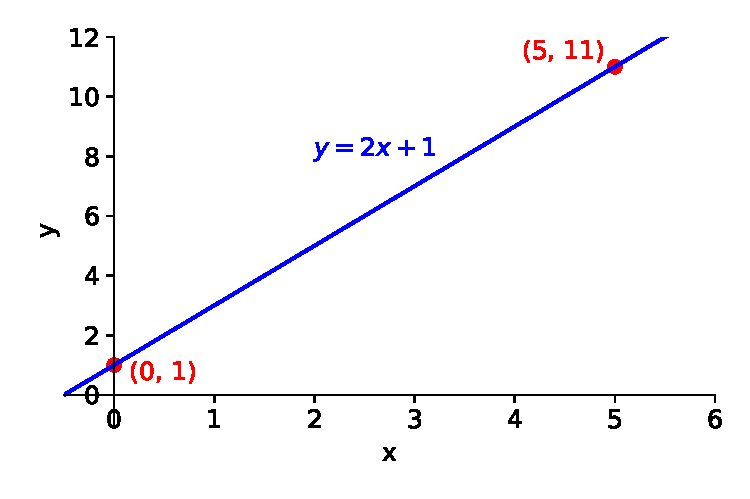
\includegraphics[width=0.5\textwidth]{Figures/example_111.pdf}
    \caption{Demonstration of plotting of $y=2x+1$ from Example 1.1.1.}
    \label{fig:straight_line_pts}
\end{figure}

Some useful properties of straight lines
\begin{itemize}
    \item Two lines are \textbf{parallel} if they have the same gradient.
    \item Two lines, with gradients $m_1$ and $m_2$, are \textbf{perpendicular} if $m_1 m_2 = -1$
    \item A \textbf{horizontal} line ($m = 0$) has equation $y = c$ 
    \item A \textbf{vertical} line ($b = 0$ in equation \eqref{line-general}) has equation $x = d$.
    \item Two straight lines cross where they have the same values of $x$ and $y$. 
\end{itemize}

\begin{example} 
Find the crossing point of the lines
\begin{align*}
    y &= x + 1 \\
    y &= -\frac{1}{2}x + 4. 
\end{align*}
\end{example} 
\fbox{
\begin{minipage}{0.95\textwidth}
We can find the crossing point $(x,y) = (\alpha, \beta)$ by solving the above equations simultaneously for $\alpha$ and $\beta$. Since the LHS is the same in both equations, we find
\begin{align*}
\alpha + 1 &= -\frac{1}{2} \alpha + 4 \\
\therefore \; \frac{3}{2} \alpha &= 3 \\
\therefore \; \alpha &= 2.
\end{align*}
Now, substituting this into \textit{e.g.} $y = x + 1$ for $x$, we get $b = 3$ and hence the crossing point is at $(x,y) = (2,3)$.
\end{minipage}}\\

\begin{definition}
\label{def:Edist}
    (Euclidean distance between two points). The \textbf{Euclidean distance} (\textit{i.e. straight line distance} between two points $(x_1, y_1)$ and $(x_2, y_2)$ in Cartesian coordinates is $d = \sqrt{(x_2-x_1)^2 + (y_2-y_1)^2}$. %This can be shown using Pythagoras rule (see figure \ref{fig:distance})/ 
\end{definition}

\subsubsection{Equation of a Circle}

The equation for a circle in Cartesian coordinates $(x,y)$ with centre at $(a,b)$ and radius $R$ is given by
\begin{align}
    \label{circle} (x - a)^2 + (y-b)^2 = R^2.
\end{align}
Using Definition \ref{def:Edist} we can see that the radius $R$ is the straight line distance between the points on the circle and its centre (which makes sense!).\\ %(see figure \ref{fig:distance})/ 

\begin{example}
    Find the centre and radius of the circle with equation
    \begin{align*}
        x^2 + 4x + y^2 - 6y = 3
    \end{align*}
\end{example}
\fbox{
\begin{minipage}{0.95\textwidth}
If we expand the equation of a circle (equation \eqref{circle}) and move the constant terms to the RHS, we find
\begin{align*}
    x^2 - 2ax + y^2 - 2by = R^2 - a^2 - b^2. \\ 
\end{align*}
Comparing the coefficients of $x$ and $y$ with the terms in the expression in the example, we see $-2a=4$ and $-2b=-6$, therefore $a=-2$ and $b=3$. Now comparing the RHS of both equations we see that $R^2-a^2-b^2=3$, which means $R^2 = 16$. Therefore, the centre of the circle is at $(x,y) = (-2,3)$ and its radius is $R=4$. 
\end{minipage}}\\

\begin{definition}
    (crossing points between a line and circle). To find the crossing points between two curves, the equations for the two curves need to be solved simultaneously. To do this, we can substitute the equation for the line (equation \eqref{line}) into the equation for the circle (equation \eqref{circle}). This leads to a quadratic equation in $x$ that can yield
    \begin{itemize}
        \item Two unique real solutions for $x$, meaning two crossing points.
        \item One (repeated) solution, meaning there is one crossing point and the line is tangent to the circle.
        \item No real solutions, meaning the line and circle do not cross.
    \end{itemize}
    %These outcomes are illustrated in figure \ref{fig:line_and_circle}.
\end{definition}

\begin{example} 
Do the following line and circle cross, if so, at what point(s)?
\begin{align*}
    y &= x + 1 \\
    (x - 1)^2 + (y-2)^2 &= 8
\end{align*}
\end{example} 
\fbox{
\begin{minipage}{0.95\textwidth}
Substituting the first equation into the second (for $y$) gives
\begin{align*}
    (x-1)^2 + (x+1-2)^2 &= 8\\
    \therefore 2(x-1)^2 &= 8\\
    \therefore x-1 &= \pm 2\\
    \therefore x &= \{-1,\; 3\}
\end{align*}
The corresponding $y$ values can be acquired easily by substituting into the equation for the line $y = x + 1$, which means there are two crossing points at $(-1,0)$ and $(3,4)$.
\end{minipage}}\\

\begin{definition}
    (lines tangent and normal to a circle). A line that passes through a point $P$ on the circle and its centre (\emph{i.e.} along the radius) is \textbf{normal} to the circle at that point. The \textbf{tangent} line is perpendicular to the normal (and therefore parallel to the circle) at the point $P$.
\end{definition}

\begin{definition}
    (perpendicular bisector of a chord). A line that passes through two points $A$ and $B$ on the circle is called a \textbf{chord}. The perpendicular bisector of this (\emph{i.e.} the line that is perpendicular to the line $AB$ and crosses it at its midpoint) will pass through the centre of the circle. %These outcomes are illustrated in figure \ref{fig:line_and_circle}.
\end{definition}

\begin{example}
    Find the equation of a circle with centre along the line $y=2x-3$ and which also passes through the two points (1,6) and (5,2). 
\end{example}
\fbox{
\begin{minipage}{0.95\textwidth}
The chord between points $A(1,6)$ and $B(5,2)$ has gradient $m = (2-6)/(5-1) = -1$. Therefore, the line perpendicular to this chord will have gradient $1$ and so equation $y = x + c$. The centre of the chord is at the point $(A+B)/2 = (3,4)$, therefore substituting $x=3$ and $y=4$ into $y = x + c$ gives $c = 1$, and so $y=x+1$ is a perpendicular bisector of the chord and so pass through the centre of the circle. 

We know that $y=2x-3$ also passes through the centre, so the point where $y=2x-3$ and $y=x+1$ cross must be the centre. Equating the RHS of each gives $2x-3=x+1$ and so $x=4$, and therefore $y=5$. Therefore, the equation will be of the form $(x-4)^2 + (y-5)^2 = R^2$. To find $R$, we can substitute in any point on the circle (as they all must satisfy this equation). Substituting in $A$ we find $(1-4)^2+(6-5)^2=R^2$ and so $R^2=10$. So, finally, the equation of the circle is given by
\begin{align*}
    (x-4)^2 + (y-5)^2 = 10.
\end{align*}
We can check this solution by substituting in the point $B$ and noting that it also satisfies the equation. 
\end{minipage}}

\newpage
\subsection{Parametric and Implicit Functions}

When discussing functions so far we have usually focused on the \textbf{explicit} form $y = f(x)$ which directly relates the value of $x$ to the corresponding value of $y$. In this section we will look at alternative ways to represent the relationships between the variables $x$ and $y$.

\subsubsection{Parametric Functions}

A parametric function introduces a \textbf{parameter} (\textit{e.g.} $t$) and expresses our variables in terms of this parameter, such that 
\begin{align}
    x = g(t) \quad \mathrm{and} \quad y = h(t). 
\end{align}
Parametric functions arise naturally in many contexts (\textit{e.g.} when measuring how two quantities $x$ and $y$ change with time $t$). They are also useful in many circumstances as a way to simplify the relationship between $x$ and $y$.\\

Note, however, that not all parametric functions can be expressed in explicit form $y = f(x)$ and often the parametric form of $x$ and $y$ means they may be restricted to certain value ranges. In general, if the equation for $x$ can be rearranged to give $t$ as a function of $x$, this can be substituted into the equation for $y$ to give the explicit form. However, this is not necessarily always the best way to find the explicit form.\\

\begin{example}
    Sodium oxide (Na$_2$O) is placed in water, each molecule of Na$_2$O reacts with H$_2$O to produce 2 molecules of sodium hydroxide (NaOH). The number of molecules of Na$_2$O and NaOH in solution with respect to time $t \geq 0$ is given by $x = x_0e^{-\alpha t}$ and $y = 2x_0(1 - e^{-\alpha t})$ respectively, where the constant $x_0$ is the initial number of molecules of Na$_2$O. Write the number of sodium hydroxide molecules $y$ as a function of the number of sodium oxide molecules $x$, noting any restrictions on $x$ and $y$. 
\end{example}
\fbox{
\begin{minipage}{0.95\textwidth}
The parametric form of $x$ can be rearranged as $\exp(-\alpha t) = x/A$ and we can substitute this into the equation for $y$ to see that $y = 2(x_0-x)$. Since $t \geq 0$, $x$, is restricted to be between $x_0$ (at $t=0$) and $0$ (as $t \rightarrow \infty$). Similarly, $y$ is restricted to be between $0$ (at $t=0$) and $2x_0$ (as $t \rightarrow \infty$). Therefore we can write $0 \leq x \leq x_0$ and $0 \leq y \leq 2x_0$.\\

We see this makes sense with the description of the reaction. At $t=0$, $x = x_0$ and so $y = 0$, as the reaction proceeds, for every molecule of $x$ that is lost, $y$ increases by 2, until eventually converging towards $x \rightarrow 0$ and $y \rightarrow 2x_0$. 
\end{minipage}}\\

\begin{example}
\label{eg:parametric_circle}
     Express the circle with centre at (2,3) and radius 4 in parametric form.
\end{example}
\fbox{
\begin{minipage}{0.95\textwidth}
The standard way to represent a circle in parametric form is to use the angle $0 \leq \theta < 2\pi$ that radius of the circle makes with the $x$-direction. All points on the circle are the same distance $R$ from the centre $(a,b)$, so we can write $x=a+R\cos\theta$ and $y=b+R\sin \theta$. Substituting in the values gives the parametric form for this case 
\begin{align*}
    x&=2+4\cos\theta\\
    y&=3+4\sin\theta.
\end{align*}
We can check this by substituting into the non-parametric form $(x-2)^2+(y-3)^2=16$. and seeing that it satisfies the equation.
\end{minipage}}\\

\subsubsection{Implicit Functions}

Implicit functions are those written in the form $g(x,y) = 0$, as opposed to explicit functions of the form $y = f(x)$. In many cases, this form is more general (\textit{e.g.} there might be multiple solutions for $y$ and expressing as $y = f(x)$ may suppose only one of them). Note, we have already seen the implicit form for a straight line in equation \eqref{line-general} and for a circle in equation \eqref{circle}.
\begin{example}
    \label{eg:ellipse} An ellipse can be written in implicit form as
    \begin{align*}
        \frac{x^2}{100} + \frac{y^2}{25} = 1.
    \end{align*}
    For $x = -10, -8, -6, 0, 6, 8, 10$ find possible values of $y$ and hence draw the ellipse.
\end{example}
\fbox{
\begin{minipage}{0.95\textwidth}
Rearranging into explicit form $y = \pm 5\sqrt{1 - x^2/100}$. Note that this is the same for $\pm x$ so substituting in $x = \pm10, \pm8, \pm6, 0$ we get $y = 0, \pm3, \pm4, \pm 5$ respectively. These points are plotted in figure \ref{fig:ellipse} along with the outline of the ellipse. 
\end{minipage}}\\

\begin{figure}[h!]
    \centering
    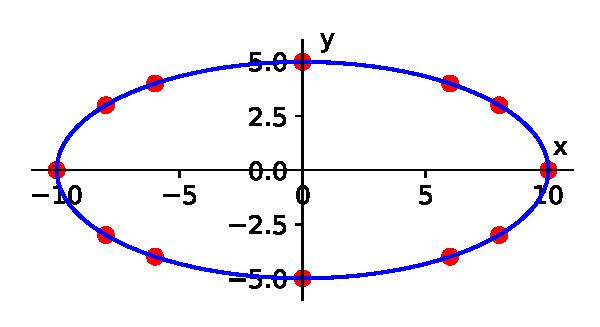
\includegraphics[width=0.5\linewidth]{Figures/example_123.pdf}
    \caption{Plot of the ellipse and calculated points in example \ref{eg:ellipse}.}
    \label{fig:ellipse}
\end{figure}


\newpage
\subsection{Partial Fraction Decomposition}

\subsubsection{Partial fractions in general}

``Partial fractions'' is a term used to describe the separation of a rational fraction (where both the numerator and denominator are both polynomials) into a sum of simplified rational fractions each with an irreducible polynomial on the denominator. It is often preferable to decompose a rational fraction into partial fractions for the purposes of differentiation or integration (which we will cover in section \ref{sec:calculus}).\\

The reverse procedure (expressing partial fractions as a single rational fraction) is much easier to achieve, as shown in the following example.

\begin{example}
    Express $1/(x+1) + 3/(x-2)$ as a single rational fraction.
\end{example}
\fbox{
\begin{minipage}{0.95\textwidth}
Multiplying the numerator and denominator of a fraction by the same expression does not change its value (except at troublesome points where the expression is 0, which we will ignore for now). So, we multiply numerator and denominator of each fraction by the denominator of the other, to get 
\begin{align*}
    &\frac{1}{x+1} + \frac{3}{x-2}\\
    &=\frac{x-2}{(x+1)(x-2)} + \frac{3(x+1)}{(x+1)(x-2)}\\
    &= \frac{4x-1}{(x+1)(x-2)}.
\end{align*}
\end{minipage}}\\

An example of partial fraction decomposition then would be to begin with $\frac{4x-1}{(x+1)(x-2)}$ and simplify it to $\frac{1}{x+1} + \frac{3}{x-2}$. Clearly, this is less straight-forward and so we need some generic rules that we can apply to solve this type of problem.\\

The process for decomposing into partial fractions depends on whether the fraction is proper or improper and whether the polynomials can be factorised.   

\begin{definition}
    (proper and improper rational fractions) A rational fraction is defined as \textbf{proper} if $d > n$ where $d$ is the degree of the polynomial in the denominator and $n$ is the degree of the polynomial in the numerator. It is improper if $n \geq d$. 
\end{definition}

\begin{example}
    Determine whether $(ax + b)^2/(cx^2 + d)$ is a proper rational fraction, where $a$, $b$, $c$, and $d$ are constants and $x$ is the independent variable.
\end{example}
\fbox{
\begin{minipage}{0.95\textwidth}
The numerator $(ax + b)^2$ is a polynomial of degree 2 (as the largest power of $x$ in the numerator is $x^2$) and the denominator $(cx^2 + d)$ is also degree 2. Therefore $d = n$ and so the fraction is improper.\\
\end{minipage}}\\

The steps for decomposing a rational fraction $f(x)/g(x)$ into partial fractions are as follows
\begin{enumerate}
    \item Factorise the polynomial denominator $g(x) = g_1(x)g_2(x)\ldots$
    \item Use this factorisation to write the functional form of the partial fractions $f_0(x) + f_1(x)/g_1(x) + f_2(x)/g_2(x) + \ldots$ using the rules in definitions \ref{def:linear_pf} -- \ref{def:improper}. 
    \item Equate both sides $f(x)/g(x) = f_0(x) + f_1(x)/g_1(x) + f_2(x)/g_2(x) + \ldots$, solve for the unknown coefficients in $f_1(x)$, $f_2(x)$, $\ldots$ by multiplying through by $g(x)$ to get a polynomial on both sides and comparing coefficients.
\end{enumerate}
This will make more sense with examples, which we can attempt once we have introduced some of the rules needed to complete step 2.

\subsubsection{Decomposition of proper fractions}
\label{sec:proper_fracs}

\begin{definition}
\label{def:linear_pf}
    (Partial fraction decomposition for proper fractions with linear factors in the denominator). If the fraction is proper and its denominator factorises into linear expressions in $x$ (\textit{i.e.} $g(x) = (x-a)(x-b)\ldots$ we can write
    \begin{align}
        \label{linear_pf} \frac{f(x)}{(x-a)(x-b)\ldots} = \frac{A}{x-a} + \frac{B}{x-b} + \ldots ,
    \end{align}
    where $A$ and $B$ are constant coefficients to be determined. 
\end{definition}

\begin{example}
    Express $(x-4)/(2x^2+5x-3)$ as partial fractions.
\end{example}
\fbox{
\begin{minipage}{0.95\textwidth}
First, we factorise the denominator to get $(x - 4)/[(x+3)(2x-1)]$, then use the rule in equation \eqref{linear_pf} to write
\begin{align*}
    \frac{x - 4}{(x+3)(2x-1)} &= \frac{A}{x+3} + \frac{B}{2x-1},\\
    \therefore x-4 &= A(2x-1) + B(x+3)
\end{align*}
Rather than comparing coefficients, in the case of two linear factors it is easier to evaluate the above at $x=-3$ and $x=1/2$ to yield $A = 1$ and $B = -1$ directly, and so
\begin{align*}
    \frac{x-4}{2x^2+5x-3} = \frac{1}{x+3} - \frac{1}{2x-1}.
\end{align*}
\end{minipage}}\\

\begin{example}
    Express $(2x^2+8x+18)/[x(x+2)(x-3)]$ as partial fractions.
\end{example}
\fbox{
\begin{minipage}{0.95\textwidth}
The denominator is already factorised into linear factors and the fraction is proper so we can use equation \eqref{linear_pf} to write
\begin{align*}
    \frac{2x^2+8x+18}{x(x+2)(x-3)} &= \frac{A}{x} + \frac{B}{x+2} + \frac{C}{x-3},\\
    \therefore 2x^2+8x+18 &= A(x+2)(x-3) + Bx(x-3) + Cx(x+2) \\
    \therefore 2x^2+8x+18 &= (A + B + C)x^2 + (-A -3B +2C) - 6A.
\end{align*}
Comparing the constant coefficients first we see $-6A=181$ and so $A=-3$. Comparing coefficients of the $x^2$ and $x$ terms then leaves
\begin{align*}
B + C &= 5\\
-3B+2C &= 5,
\end{align*}
which yields $C = 4$ and $B=1$. Therefore
\begin{align*}
    \frac{2x^2+8x+18}{x(x+2)(x-3)} &= -\frac{3}{x} + \frac{1}{x+2} + \frac{4}{x-3}.
\end{align*}
\end{minipage}}\\

\begin{definition}
    (Partial fraction decomposition for proper fractions with repeated linear factors in the denominator). If the fraction is proper and its denominator contains a linear fractor that is repeated (\textit{i.e.} $g(x) = (x-a)^2\ldots$ we can write
    \begin{align}
        \label{linear_repeat_pf} \frac{f(x)}{(x-a)^2\ldots} = \frac{A}{x-a} + \frac{B}{(x-a)^2} + \ldots,
    \end{align}
    where $A,B$ are constant coefficients to be determined. 
\end{definition}

\begin{example}
    Decompose $(2x - 5)/(x^2-6x+9)$ into partial fractions.
\end{example}
\fbox{
\begin{minipage}{0.95\textwidth}
First, factorise the denominator and then use the rule in equation \eqref{linear_repeat_pf} to write
\begin{align*}
    \frac{2x-5}{(x-3)^2} &= \frac{A}{x-3}+\frac{B}{(x-3)^2}\\
    \therefore 2x - 2 &= A(x-3) + B\\
    \therefore 2x - 2 &= Ax + (B - 3A)
\end{align*}
and so comparing coefficients gives $A = 2$ and $B-3A=-5$, therefore $B=1$, and so 
\begin{align}
    \frac{2x - 5}{x^2-6x+9} = \frac{2}{x-3} + \frac{1}{(x-3)^2}.
\end{align}
\end{minipage}}\\

\begin{definition}
    (Partial fraction decomposition for proper fractions with quadratic factors in the denominator). If the fraction is proper and one of the factors of the denominator is an irreducible quadratic in $x$ (\textit{i.e.} $g(x) = (ax^2+bx+c)\ldots$ then
    \begin{align}
        \label{quadratic_pf} \frac{f(x)}{(ax^2+bx+c)\ldots} = \frac{Ax+B}{ax^2+bx+c} + \ldots,
    \end{align}
    where $A,B$ are constant coefficients to be determined. 
\end{definition}

\begin{example}
    Express $x^2/(x-1)(x^2+3x-3)$ as a partial fraction.
\end{example}
\fbox{
\begin{minipage}{0.95\textwidth}
We see that $x^2+3x-3$ cannot be factorised and so the denominator cannot be factorised further and so we use the rule in equation \eqref{quadratic_pf} to write
\begin{align*}
    \frac{x^2}{(x-1)(x^2+3x-3)} &= \frac{A}{x-1} + \frac{Bx+C}{x^2+3x-3}\\
    \therefore x^2 &= A(x^2+3x-3) + (Bx+C)(x-1)\\
    \therefore x^2 &= (A+B)x^2 + (3A+B+C)x - (C+3A)
\end{align*}
Comparing coefficients we see that $C=-3A$, and so $B=0$. Therefore $A=1$ and $C=-3$, giving  
\begin{align*}
    \frac{x^2}{(x-1)(x^2+3x-3)} = \frac{1}{x-1} - \frac{3}{x^2+3x-3}.
\end{align*}
\end{minipage}}\\

\subsubsection{Decomposition of improper fractions}

\begin{definition}
\label{def:improper}
    (partial fraction decomposition of improper fractions). For improper fractions, where $n > d$, we need to account for the extra orders of the polynomial in the numerator by adding a polynomial to the RHS of order $n-d$, i.e.
    \begin{align}
        \label{improper} \frac{f(x)}{g(x)} = a_0 + a_1x + \ldots a_{n-d} x^{n-d} + \ldots
    \end{align}
    where the constants $a_0, \ldots, a_{n-d}$ are to be determined. what follows this polynomial on the RHS depends on the form of $g(x)$, using the same rules as for proper fractions in section \ref{sec:proper_fracs}.
\end{definition}

\begin{example}
    Express $3(x+1)^2/(x^2+x-2)$ as partial fractions.
\end{example}
\fbox{
\begin{minipage}{0.95\textwidth}
First we factorise the denominator to $(x - 1)(x + 2)$. The numerator and denominator have the same order, so the fraction is improper with $n-d=0$. Using the rules in \eqref{improper} and \eqref{linear_pf} we can write
\begin{align*}
    \frac{3(x+1)^2}{(x - 1)(x + 2)} &= A + \frac{B}{x-1} + \frac{C}{x+2}\\
    \therefore 3x^2 + 6x + 3 &= A(x^2 + x -2) + B(x+2) + C(x-1) \\
    \therefore 3x^2 + 6x + 3 &= Ax^2 + (A+B+C)x + (-2A+2B-C).
\end{align*}
Comparing $x^2$ coefficients we find $A = 3$, and so comparing the $x^1$ and $x^0$ coefficients we have $B+C=3$ and $2B-C=9$. This gives $C = -1$ and $B = 4$ and so
\begin{align*}
    \frac{3(x+1)^2}{x^2+x-2} = 3 + \frac{4}{x-1} - \frac{1}{x+2}
\end{align*}
\end{minipage}}\\

\begin{example}
    Write the partial fractions form of the following
    \begin{align*}
        \frac{5x^6 - 50x^5 + 386x^4 - 1074x^3 + 644x^2 + 1174x - 1354}{(x-2)^2(x^2-6x+50)},
    \end{align*}
    but do not find the values of the coefficients.
\end{example}
\fbox{
\begin{minipage}{0.95\textwidth}
The polynomial in the numerator is order 6, while the denominator is order 4, so from definition \ref{def:improper} we know the RHS must contain a quadratic. In the denominator, the first linear terms are repeated, so we use the rule in equation \ref{linear_repeat_pf}, and he quadratic expression cannot be factorised so we use the rule in equation \ref{quadratic_pf}. Putting all this together we see that the partial fraction decomposition must have the following form
\begin{align*}
    Ax^2 + Bx + C + \frac{D}{x-2} + \frac{E}{(x-2)^2} + \frac{Fx+G}{x^2-6x+50}.
\end{align*}
\end{minipage}}



% % Transcription draft based on Section 2 slides and video examples
\section{Differentiation}

\begin{ILOssec}
    \item \ILOc
\end{ILOssec}

\subsection{Maxima and minima of functions}
\label{sec:min_max}

\begin{learningoutcomes}
\item Calculate the derivative of basic mathematical functions
\item Identify local and global maxima and minima of a function
\end{learningoutcomes}

\subsubsection{Reminder of basic differentiation}
\textbf{What is the derivative?} We have calculated the gradient of a straight line as
\[
m=\frac{\Delta y}{\Delta x}.
\]
The derivative of a function $f(x)$ is the gradient at a point (i.e. as the change in $x$ gets infinitesimally small)
\begin{equation}
    f'(x)=\lim_{h\to0}\frac{f(x+h)-f(x)}{h}.
\end{equation}


Another way to imagine this is demonstrated in figure \ref{fig:diff_zoom}. As we ``zoom in'' on any smooth function, it looks more like a straight line with gradient equivalent to the tangent line at that point, \textit{i.e.} the derivative. Some common derivatives of functions are given in table \ref{tab:derivatives}. 

\begin{figure}[h!]
    \centering
    \iflatexml
        \<div id="tangent-animation">\</div>
        \<script src="tangent-animation.js">\</script>
    \else
        \subfig{0.3}{Figures/Section2/plot_h_0.png}{Zoomed out, $h=1$.}
        \subfig{0.3}{Figures/Section2/plot_h_80.png}{Zooming in, $h=0.1$.}
        \subfig{0.3}{Figures/Section2/plot_h_210.png}{Zoomed in, $h=0.01$.}
    \fi
    \caption{The straight line between two points on the curve $\sin x$ gets closer to a tangent to the curve as we zoom in and reduce $h$, becoming a better approximation of the derivative at the left-hand point, which remains fixed.}
    \label{fig:diff_zoom}
\end{figure}

{\renewcommand{\arraystretch}{1.75}\begin{table}[ht]
    \centering
    \begin{tabular}{|c|c|} \hline
    Function $y = f(x)$ & Derivative ${\rm d}y/{\rm d}x = f'(x)$ \\ \hline
    $x^n$ & $nx^{n-1}$\\
    $\ln x$ & $\displaystyle\frac{1}{x}$\\
    $e^x$ & $e^x$\\
    $\sin x$ & $\cos x$\\
    $\cos x$ & $-\sin x$\\
    $\tan x$ & $\sec^2 x$\\
    $\sin^{-1} x$ & $\displaystyle\frac{1}{\sqrt{1-x^2}}$\\
    $\cos^{-1} x$ & $\displaystyle-\frac{1}{\sqrt{1-x^2}}$\\
    $\tan^{-1} x$ & $\displaystyle\frac{1}{1+x^2}$\\\hline
    \end{tabular}
    \caption{Some common functions and their derivatives (see the mathematical formula tables for more standard derivatives).}
    \label{tab:derivatives}
\end{table}}

\textbf{The second derivative.} When a function is differentiated, the resulting derivative is also a function. It can, itself be differentiated to form the second derivative, denoted as
\[
    \der{^2y}{x^2} \qquad \mathrm{or} \qquad f''(x)
\]

\subsubsection{Local maxima and minima}

\textbf{Stationary points.} A point where $f'(x)=0$ is called a stationary point. It may represent a place where the function is a maximum or a minimum, but it could represent something else (see figure \ref{fig:stat_points}). To find stationary points, we need to solve $f'(x)=0$ for $x$, there could be
\begin{itemize}
    \item no stationary points
    \item one stationary point
    \item several stationary points.
\end{itemize}

\begin{figure}[h!]
    \centering
    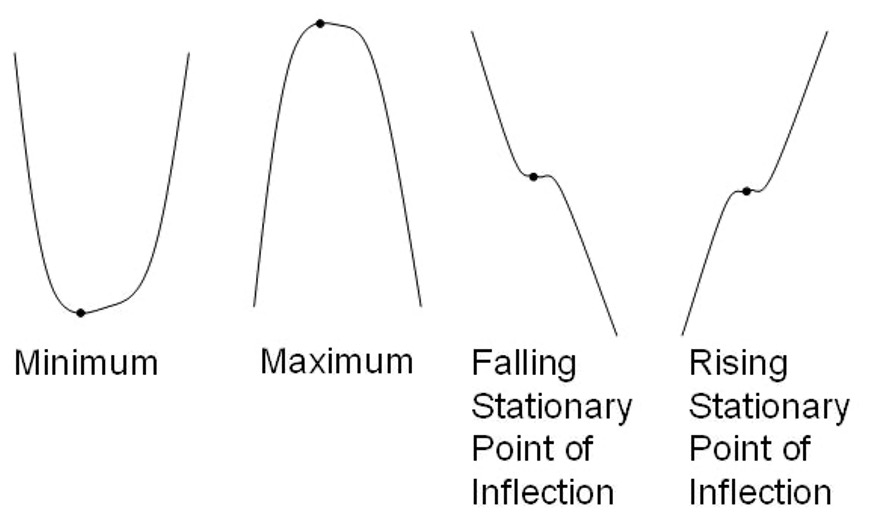
\includegraphics[width=0.5\linewidth]{Figures/Section2/212_stat_points.jpg}
    \caption{Sketch of the four types of stationary point.}
    \label{fig:stat_points}
\end{figure}

\textbf{The first derivative test.} To use this test to classify a stationary point at $x=x_0$, 
\begin{enumerate}
    \item evaluate $f'(x)$ at two points either side of $x_0$, \emph{i.e.} $f'(x_0-h)$ and $f'(x_0+h)$ for small $h$. Make sure $h$ is small enough so that $x_0 \pm h$ does not cross any other stationary points.
    \item Drawing the line \textbackslash for a negative value, / for a positive value and -- for the stationary point itself, sketch how the function looks around the stationary point (\textit{e.g.} a minimum will be \textbackslash -- /, and a maximum  / --\textbackslash).
\end{enumerate}

\textbf{The second derivative test.} To use this test to classify a stationary point at $x=x_0$, evaluate the second derivative $f''(x)$ at $x=x_0$.
\begin{itemize}
    \item If $f''(x_0) > 0$, the point is a minimum.
    \item If $f''(x_0) < 0$, the point is a maximum.
    \item If $f''(x_0) = 0$, the test is inconclusive. Fall back on the first derivative test. 
\end{itemize}

\goodbreak
\begin{example}[Lecture]
Find any stationary points for the function
\[
f(x)=2x^3-9x^2+5 \, .
\]
Use the first derivative test to classify them as maxima, minima or points of inflection. Check this using the second derivative test.
\end{example}
%
\begin{solution}
Find the first derivative
\[
f'(x)=\blank{6x^2-18x}.
\]
Solve for $f'(x)=0$.
Stationary points are at
\[
x=\blank{0}\qquad \text{and} \qquad x=\blank{3}.
\]
First derivative test for $x=0$:\par
\vspace{4mm}
\begin{tabular}{|p{10mm}|p{10mm}|p{10mm}|p{10mm}|}\hline
    $x$ & -1 & 0 & 1\\\hline
    $f'(x)$ & \blankpar{24} & 0 & \blankpar{-12}\\\hline
    sketch & \blankpar{/} & -- & \blankpar{\textbackslash}\\\hline
\end{tabular}

\vspace{4mm}
First derivative test for $x=3$:\par
\vspace{4mm}
\begin{tabular}{|p{10mm}|p{10mm}|p{10mm}|p{10mm}|}\hline
    $x$ & 2 & 3 & 4\\\hline
    $f'(x)$ & \blankpar{-12} & 0 & \blankpar{24}\\\hline
    sketch & \blankpar{\textbackslash} & -- & \blankpar{/}\\\hline
\end{tabular}
\vspace{4mm}

Find the second derivative:
\[
f''(x)=\blank{12x-18}.
\]
\[
f''(0)=\blank{-18},\qquad f''(3)=\blank{18}.
\]
Hence $x=\blank{0}$ is a \blankpar{maximum} and $x=\blank{3}$ is a \blankpar{minimum}.
\end{solution}

\subsubsection{Maximum and minimum values over an interval}

Consider the function $f(x)$ in figure \ref{fig:minmax}(a); where is the maximum? Where is the minimum? We can see there are stationary points at $a$ (\textbf{local} maximum) and $b$ (\textbf{local} minimum), but these are not the greatest or smallest values of $f(x)$ over the interval shown. In fact, the minimum over the interval shown is at the left boundary, and the maximum at the boundary. 

\begin{figure}[h!]
    \centering
    \subfig{0.8}{./Figures/Section2/213_minmax.png}{A function with local minima/maxima and greatest/least values labelled.}
    \hfill
    \subfig{0.6}{./Figures/Section2/213_point_types.jpg}{Sketch showing the different candidate points for the greatest/least values of a function in an interval.}
    \caption{}
    \label{fig:minmax}
\end{figure}

The greatest/least values of a function within an interval can occur at the following points (labelled on figure \ref{fig:minmax}(b))
\begin{enumerate}[label=(\Alph*)]
    \item Stationary points (local maxima/minima),
    \item Ends of the interval for $x$,
    \item Where $f(x)$ becomes infinite for finite $x$,
    \item Where $f(x)$ or $f'(x)$ does not exist,
    \item As $x$ becomes infinite (positive or negative).
\end{enumerate}
Such points are often referred to as \textbf{critical points}. It is a case of checking all such points in the interval. 

\goodbreak
\begin{example}[Lecture]
Find the maximum and minimum values of the function
\[
p(x)=2x^3-3x^2-36x+13
\]
on the interval $-4\leq x\leq6$.
\end{example}
%
\begin{solution}
Find first derivative
\[
p'(x)=\blank{6x^2-6x-36}.
\]
Solve for $p'(x)=0$.
\begin{align*}
    \blank{6(x^2-x-6)}&=0\\
    \blank{(x-3)(x+2)}&=0
\end{align*}
Stationary points are at $x=\blank{-2}$ and $x=\blank{3}$.

Values at stationary points:
\[
p(\blank{-2})=\blank{57},\qquad p(\blank{3})=\blank{-68}.
\]
The function $p(x)$ is continuous and finite and the bounds are finite. So just need to check the edges of the domain:
\[
p(-4)=\blank{-19},\qquad p(6)=\blank{121}.
\]
Maximum value of $\blank{121}$ at $x=\blank{6}$. Minimum value of $\blank{-68}$ at $x=\blank{3}$.
\end{solution}

\goodbreak
\begin{example}[Video]
A bioreactor produces biomass at a rate of roughly
\[
b(\omega)=3+\omega \quad [\mathrm{kg/h}],
\]
which increases with the stirring rate $\omega\geq0$ $[\mathrm{rpm}]$.
The cost of running the reactor also increases with $\omega$, roughly given by
\[
c(\omega)=72+\frac{1}{3}\omega^2 \quad [\text{\pounds}/\mathrm{h}].
\]
Find the stirring rate that optimises production efficiency (i.e. kg of biomass per \pounds$\;$spent), and the associated production efficiency.
\textbf{Note:} This can be completed once we have covered the quotient rule in section \ref{sec:quotient}).
\end{example}
%
\begin{solution}
The production efficiency (in kg of biomass per \pounds$\;$spent) is given by
\[
f(\omega)=\blank{\frac{b(\omega)}{c(\omega)}}=\blank{\frac{3+\omega}{72+\frac{1}{3}\omega^2}}.
\]
The optimal efficiency will be achieved when $f(\omega)$ is a maximum. Find the stationary points $f'(\omega)=0$, using the quotient rule:
\[
f'(\omega)=\blank{\frac{\left(72+\frac{1}{3}\omega^2\right)-(3+\omega)\frac{2}{3}\omega}{\left(72+\frac{1}{3}\omega^2\right)^2}}=0.
\]
\[
\blank{72+\frac{1}{3}\omega^2-2\omega-\frac{2}{3}\omega^2}=0.
\]
Rearranging there is a stationary point when
\[
\blank{\omega^2+6\omega-216=0}.
\]
Factorising (or using the quadratic equation)
\[
\blank{(\omega+18)(\omega-12)=0}.
\]
Since $\omega\geq0$, we have an optimal stirring rate of $\omega=\blank{12}$ $[\mathrm{rpm}]$.
Substituting this back into the equation for $f$, we get a production efficiency of
\[
f=\blank{\frac{3+12}{72+144/3}=\frac{15}{120}=\frac{1}{8}}\quad [\mathrm{kg}/\text{\pounds}].
\]
We can check this is indeed the maximum over the domain by checking $f(\omega=0) = \blank{\frac{1}{24}}$ and also $\lim_{\omega\to\infty}f(\omega) = \blank{0}$ are both \blankpar{less than} the value at the stationary point.
\end{solution}

\begin{recap}{\ref{sec:min_max}}
\item The \textbf{derivative} of a function is its gradient with respect to its variable.
\item \textbf{Local stationary points} can be found by solving $f'(x)=0$.
\item A stationary point $x_0$ is a \textbf{maximum} if $f''(x_0)<0$ and \textbf{minimum} if $f''(x_0)>0$.
\item If $f''(x_0)=0$, use the \textbf{first derivative test} instead.
\item The max and min over an interval \textbf{might not be stationary points}.
\end{recap}

\goodbreak
\subsection{The product, quotient and chain rules}
\label{sec:prod_quo_chain}

\begin{learningoutcomes}
\item Identify when to use the chain, product, or quotient rules
\item Calculate the derivatives of functions using the chain, product, or quotient rules, where appropriate
\end{learningoutcomes}

\subsubsection{The chain rule}

Consider the function
\[
f(x)=(\sin x)^2.
\]
This is a combination of two functions i.e. start with $x$, take the sine and then square it.
\[
x \quad \xrightarrow{\text{Take the sine}} \quad \sin x
\quad \xrightarrow{\text{Square it}} \quad (\sin x)^2.
\]
The inner function is $g(x)=\sin x$ and the outer function is
$h(u)=u^2$.

The chain rule tells us how to differentiate a function of a function. If $f(x)=h(u)$ where $u=g(x)$,
\begin{equation}
\label{eq:chain}  \der{f}{x} = \der{h}{u} \cdot \der{g}{x}\, ,
\end{equation}
or in alternative notation
\[
    f'(x)=h'(u)g'(x) \, ,
\]
\textit{i.e.} differentiate the outer function and multiply by the derivative of the inner function.

For the function $f(x)=(\sin x)^2$, the inner function is $u=g(x)=\sin x$. The outer function is $h(u)=u^2$. Using equation \eqref{eq:chain},
\[
f'(x)=h'(u)g'(x)=2u\cos x.
\]
Expressing in terms of $x$,
\[
f'(x)=2\sin x\cos x.
\]

\goodbreak
\begin{example}[DIY]
\label{ex:chain}
Differentiate
\[
p(t)=(t^2+1)^3
\]
using the chain rule.
\end{example}
%
\begin{blanksol}
\[
p'(t)=6t(t^2+1)^2.
\]
Let $f(t)=t^2+1$, then $p(t)=f(t)^3$. The derivative of $f(t)$ is $f'(t)=2t$. Using the chain rule
\[
p'(t)=3f'(t)f(t)^2=6t(t^2+1)^2.
\]
\end{blanksol}

Compare the solution in example \ref{ex:chain} to the result by expanding the brackets
\begin{align*}
p(t)&=(t^2+1)^3\\
&=(t^4+2t^2+1)(t^2+1)\\
&=t^6+3t^4+3t^2+1
\end{align*}
then, taking the derivative
\begin{align*}
p'(t)&=6t^5+12t^3+6t\\
&=6t(t^4+2t^2+1)\\
&=6t(t^2+1)^2.
\end{align*}
Compare this to your solution to example \ref{ex:chain}, did you get the same result? Clearly, the chain rule is more efficient. 

\textbf{Repeated chain rule.} Note the chain rule can be applied repeatedly. Consider,
\[
q(x)=e^{\sin(x^2+3)}.
\]
Write $p(x)=\sin(x^2+3)$ so that $q(x)=\exp[p(x)]$. Then, using the chain rule 
\[
q'(x)=p'(x)\exp[p(x)]
\]. 
To find $p'(x)$ use the chain rule again. Let $f(x)=x^2+3$ so $f'(x)=2x$. Then 
\[
p'(x)=f'(x)\cos f(x) \, ,
\]
and so $p'(x)=2x\cos(x^2+3)$. Using the expression for $q'(x)$ we get
\[
q'(x)=2x\cos(x^2+3)e^{\sin(x^2+3)}\, .
\]

\goodbreak
\begin{example}[Video]
\begin{enumerate}[label=(\alph*)]
    \item Find the derivative of
            \[
            y=e^{3(1-g^2(x))}
            \]
    in terms of the unknown function $g(x)$ and its derivative $g'(x)$.
    \item When $g(x)=\cos x$, what is $y'$?
\end{enumerate}
\end{example}
%
\begin{solution}
(a) First define
\[
h(x)=\blank{3(1-g^2)=3-3g^2},
\]
then
\[
h'(x)=\blank{-6gg'}.
\]
And so
\[
\blank{y'=h'e^h=-6gg'e^{3(1-g^2)}}.
\]

(b) If $g(x)=\cos x$ then $g'(x)=\blank{-\sin x}$ and therefore
\begin{align*}
y'&=\blank{-6gg'e^{3(1-g^2)}}\\
&=\blank{6\sin x\cos x\,e^{3(1-\cos^2x)}}\\
&=\blank{6\sin x\cos x\,e^{3\sin^2x}}.
\end{align*}
\end{solution}

\textbf{The Chain Rule and Linear Functions.} Consider the following functions and how to differentiate them.
\[
f(x)=\sin\left(4x+\frac{\pi}{2}\right)
\]
\[
g(x)=5e^{2x-9}
\]
\[
h(x)=7\ln(6-2x)
\]
\[
p(x)=(7x+9)^{10}.
\]

Each of these functions can be differentiated using the chain rule \textit{e.g.}
\[
f(x)=\sin\left(4x+\frac{\pi}{2}\right)
\]
\[
f'(x)=\cos\left(4x+\frac{\pi}{2}\right)\times4
\]
\[
=4\cos\left(4x+\frac{\pi}{2}\right).
\]

Each of these functions is of the form
\[
f(ax+b)
\]
and has derivative
\[
af'(ax+b).
\]

\goodbreak
\begin{example}[Lecture]
Differentiate
\[
r(x)=2\cos(5x-\pi)
\]
and
\[
p(x)=\ln(2x+1).
\]
\end{example}
%
\begin{solution}
\[
r'(x)=\blank{-10\sin(5x-\pi)}.
\]
\[
p'(x)=\blank{\frac{2}{2x+1}}.
\]
\end{solution}

\subsubsection{The product rule}

Consider the function
\[
f(x)=x\sin x.
\]
This is a product of two functions $u(x)=x$ and $v(x)=\sin x$. The product rule enables the differentiation of a product of two functions.

If
\[
f(x)=u(x)v(x),
\]
then the \textbf{product rule} states
\begin{equation}
    \der{}{x}(uv)=v\frac{{\rm d}u}{{\rm d}x}+u\frac{{\rm d}v}{{\rm d}x}.
\end{equation}

or, in alternative notation
\[
f'(x)=u'(x)v(x)+u(x)v'(x),
\]
\emph{i.e.} multiply each function by the derivative of the other and add together. Note, it \textbf{does not matter} which function is $u$ and which function is $v$.

In the case $f(x)=x\sin x$, let $u(x)=x$ and $v(x)=\sin x$. Then $u'(x)=1$ and $v'(x)=\cos x$. Using $f'(x)=uv'+vu'$,
\[
f'(x)=x\cos x+\sin x.
\]

\goodbreak
\begin{example}[Lecture]
Differentiate
\[
g(x)=3x^2\ln x
\]
using the product rule.
\end{example}
%
\begin{solution}
Let $u(x)=\blank{3x^2}$ and $v(x)=\blank{\ln x}$. Then $u'(x)=\blank{6x}$ and $v'(x)=\blank{1/x}$. Using the product rule $g'(x)=uv'+u'v$,
\[
g'(x)=\blank{3x+6x\ln x}=\blank{3x(1+2\ln x)}.
\]
\end{solution}

\textbf{The product rule for products of three or more functions.} Consider
\[
f(x)=u(x)v(x)w(x)
\]
and make the substitution
\[
s(x)=v(x)w(x)
\]
so that
\[
f(x)=u(x)s(x).
\]

Thus
\[
f'(x)=u's+us'\, .
\]
Using the product rule for $s(x)=v(x)w(x)$:
\[
s'(x)=v'w+vw'\,.
\]
Substituting into $f'(x)$:
\begin{align}
f'(x)&=u'vw+u(v'w+vw')\\
&=u'vw+uv'w+uvw'
\end{align}
gives the sum of three terms. Each is the product of two functions multiplied by the derivative of the third function.

\goodbreak
\begin{example}[Video]
Differentiate
\[
g(x)=x^2e^x\sin(\pi x)
\]
using the product rule.
\end{example}
%
\begin{solution}
Define $u(x)=x^2$, $v(x)=e^x$, and $w(x)=\sin(\pi x)$, so that $g=uvw$.

The product rule for three functions states that
\[
g'=u'vw+uv'w+uvw'.
\]
Find the derivatives of $u$, $v$, and $w$:
\[
u'=\blank{2x},
\qquad
v'=\blank{e^x},
\qquad
w'=\blank{\pi\cos(\pi x)}.
\]
And substitute them into the expression for $g'$:
\[
\blank{g'=2xe^x\sin(\pi x)
+x^2e^x\sin(\pi x)
+x^2e^x\pi\cos(\pi x)}.
\]
Which can be factorised as
\[
\blank{g'=xe^x\left[2\sin(\pi x)+x\sin(\pi x)+\pi x\cos(\pi x)\right]}
\]
\[
\blank{=xe^x\left[(x+2)\sin(\pi x)+\pi x\cos(\pi x)\right]}.
\]
\end{solution}

\subsubsection{The quotient rule}
\label{sec:quotient}

Consider the function
\[
f(x)=\frac{\sin x}{x}.
\]
This is a quotient of two functions \textit{i.e.} one function divided by another. The quotient rule enables the differentiation of a quotient of two functions.

If
\[
f(x)=\frac{u(x)}{v(x)},
\]
then the quotient rule states
\begin{equation}
    \der{}{x}\left(\frac{u}{v}\right)
= \frac{v\dfrac{{\rm d}u}{{\rm d}x}-u\dfrac{{\rm d}v}{{\rm d}x}}{v^2} \, .
\end{equation}
or in alternative notation
\[
f'(x)=\frac{u'v-uv'}{v^2}.
\]
Unlike the product rule, it is now \textbf{critical} which is $u$ and which is $v$.

\goodbreak
\begin{example}[Lecture]
Differentiate
\[
g(x)=\frac{\ln x}{x^2}
\]
by two methods:
\begin{enumerate}
\item[(a)] Using the quotient rule
\item[(b)] Writing as $g(x)=x^{-2}\ln x$ and using the product rule.
\end{enumerate}
\end{example}
%
\begin{solution}
(a) Let $u(x)=\ln x$ and $v(x)=x^2$. Then
\[
u'(x)=\blank{\frac{1}{x}}
\qquad\text{and}\qquad
v'(x)=\blank{2x}.
\]
Using the quotient rule
\[
g'(x)=\frac{u'v-uv'}{v^2}=\blank{\frac{x-2x\ln x}{x^4}}
\]
\[
=\frac{1-2\ln x}{x^3}.
\]

(b) Now let $u(x)=\ln x$ and $v(x)=x^{-2}$. Then
\[
u'(x)=\blank{\frac{1}{x}}
\qquad\text{and}\qquad
v'(x)=\blank{-2x^{-3}}.
\]
Using the product rule
\[
g'(x)=u'v+uv'=\blank{\frac{1}{x}x^{-2}-2x^{-3}\ln x}
\]
\[
=\blank{\frac{1-2\log x}{x^3}}.
\]
\end{solution}

\goodbreak
\begin{example}[Video]
Differentiate $x$ with respect to $t$, where
\[
x=\frac{e^{2t}\sin(t^3)}{t}.
\]
\end{example}
%
\begin{solution}
Define $u(t)=e^{2t}\sin(t^3)$ and $v(t)=t$ and find their derivatives.

For $u'(t)$, we need to use the product rule and chain rule:
\begin{align*}
u'(t)&=\blank{2e^{2t}\sin(t^3)+e^{2t}3t^2\cos(t^3)}\\
&=\blank{e^{2t}\left[2\sin(t^3)+3t^2\cos(t^3)\right]}.
\end{align*}
and
\[
v'(t)=\blank{1}\, .
\]
The quotient rule states
\[
x'=\frac{u'v-v'u}{v^2}.
\]
Substituting in the expressions for $u$, $v$, $u'$, and $v'$ gives
\begin{align*}
x'&=\blank{\frac{e^{2t}\left[2\sin(t^3)+3t^2\cos(t^3)\right]t-e^{2t}\sin(t^3)}{t^2}}\\
&=\blank{e^{2t}\left[\frac{2t-1}{t^2}\sin(t^3)+3t\cos(t^3)\right]}\,.
\end{align*}
\end{solution}

\begin{recap}{\ref{sec:prod_quo_chain}}
\item The \textbf{chain rule}: if $f(x)=h(u)$ where $u=g(x)$ then
\[
f'(x)=h'(u)g'(x).
\]
\item The \textbf{product rule}: if $f(x)=u(x)v(x)$ then
\[
f'(x)=u'v+uv'.
\]
\item The \textbf{quotient rule}: If $f(x)=u(x)/v(x)$ then
\[
f'(x)=\frac{u'v-uv'}{v^2}.
\]
\end{recap}

\goodbreak
\subsection{Implicit, logarithmic, and parametric differentiation}
\label{sec:other_diff_rules}

\begin{learningoutcomes}
\item Identify when to use implicit, logarithmic, and parametric differentiation
\item Calculate the derivatives of functions using implicit, logarithmic, and parametric differentiation, where appropriate
\end{learningoutcomes}

\subsubsection{Implicit differentiation}

Consider the implicit relation
\[
x^2+y^2=25.
\]
Although written in implicit form, it can be differentiated. It is important to know which variable we are differentiating with respect to. In this case, we want to find ${\rm d}y/{\rm d}x$.

Differentiate term-by-term with respect to $x$:
\begin{itemize}
\item The derivative of $x^2$ is $2x$
\item Using the chain rule, the derivative of $y^2$ is $2y\der{y}{x}$
\item The derivative of 25 is zero
\end{itemize}
Therefore, we have
\[
2x+2y\der{y}{x}=0.
\]
Which rearranges to
\[
\der{y}{x}=-\frac{x}{y}.
\]
This is an example of \textbf{implicit differentiation}.

The second derivative can also be found by repeating the process. Starting with $x^2+y^2=25$ and differentiating we get
\[
2x+2y\der{y}{x}=0.
\]
\begin{itemize}
\item Differentiating $2x$ gives 2
\item Using the product rule, differentiating $2y\der{y}{x}$ gives $2\left(\der{y}{x}\right)^2+2y\der{^2y}{x^2}$
\end{itemize}
So, we find
\[
2+2\left(\der{y}{x}\right)^2+2y\der{^2y}{x^2}=0
\]
or
\[
\der{^2y}{x^2}=-\frac{1+\left(\der{y}{x}\right)^2}{y}.
\]
Substituting in the result from before (${\rm d}y/{\rm d}x=-x/y$), this reduces to
\[
\der{^2y}{x^2}=-\frac{1}{y}-\frac{x^2}{y^3}.
\]

Alternatively, we could start with the result for ${\rm d}y/{\rm d}x$, \emph{i.e.}
\[
\der{y}{x}=-\frac{x}{y}.
\]
Use the quotient rule to differentiate, with $u=-x$ and $v=y$, so $u'=-1$ and $v'=y'$:
\[
\der{^2y}{x^2}=\frac{u'v-v'u}{v^2}=\frac{-y+xy'}{y^2}.
\]
Substituting in the previous result $y'=-x/y$ gives
\[
\der{^2y}{x^2}=\frac{-y-x^2/y}{y^2}=-\frac{1}{y}-\frac{x^2}{y^3},
\]
\emph{i.e.} the same result as before.

\goodbreak
\begin{example}[Lecture]
If
\[
x^4+2xy+y^4=1,
\]
find the derivatives ${\rm d}y/{\rm d}x$ and $d^2y/{\rm d}x^2$ at the point $x=1$, $y=0$.
\end{example}
%
\begin{solution}
Differentiate the equation with respect to $x$ and rearrange for ${\rm d}y/{\rm d}x$.
\begin{align*}
\blank{4x^3 + 2y + 2x\der{y}{x} + 4y^3\der{y}{x}}&=\blank{0}\\
\blank{(4y^3+2x)\der{y}{x}} &= \blank{-(4x^3 + 2y)}\\
\der{y}{x}&=\blank{-\frac{4x^3+2y}{2x+4y^3}}
\end{align*}
Differentiate the original expression again and rearrange for $d^2y/{\rm d}x^2$.
\begin{align*}
\blank{12x^2 + 4\der{y}{x} + 2x\der{^2y}{x^2} + 12y^2\left(\der{y}{x}\right)^2 + 4y^3\der{^2y}{x^2}} = \blank{0}\\
\blank{(2x+4y^3)\der{^2y}{x^2}} = \blank{-12y^2\left(\der{y}{x}\right)^2 - 4\der{y}{x} - 12x^2}\\
\therefore \; \der{^2y}{x^2}=\blank{-\frac{12x^2+4y'+12y^2(y')^2}{2x+4y^3}}.
\end{align*}
At $x=1$ and $y=0$,
\[
\der{y}{x}=\blank{-\frac{4\times 1^3}{2\times 1}} = \blank{-2}
\]
Using this in the expression for the second derivative, we find that at $x=1$ and $y=0$,
\[
\der{^2y}{x^2}=\blank{-\frac{12\times1^2+ 4\times(-2)}{2\times 1}} = \blank{-2}\,.
\]
\end{solution}

\subsubsection{Logarithmic differentiation}

Logarithmic differentiation is a special case of implicit differentiation. It can make derivatives simpler by taking advantage of the properties of logarithms, such as
\begin{itemize}
\item Transforming products into sums: $\ln(ab)=\ln a+\ln b$
\item Transforming powers into coefficients: $\ln(x^n)=n\ln x$
\end{itemize}

E.g. consider a function of the form
\[
y=f(x)g(x)h(x).
\]
On taking the logarithm of the absolute value of both sides,
\[
\ln |y|=\ln|fgh|
\]
\[
=\ln| f|+\ln |g|+\ln |h|.
\]
Using implicit differentiation, the derivative of the left-hand side is
\[
\der{}{x}(\ln |y|)=\frac{1}{y}\der{y}{x}.
\]
Differentiating both sides and using this rule gives
\[
\frac{1}{y}\der{y}{x}=\frac{f'}{f}+\frac{g'}{g}+\frac{h'}{h}.
\]

Therefore, using logarithmic differentiation
\[
y=f(x)g(x)h(x)
\]
gives
\[
\der{y}{x}=y\left(\frac{f'(x)}{f(x)}+\frac{g'(x)}{g(x)}+\frac{h'(x)}{h(x)}\right).
\]
This could have also been arrived at by rearranging the product rule for three functions.

\goodbreak
\begin{example}[Lecture]
Use logarithmic differentiation to find the derivative of
\[
y=\frac{\sqrt{(x+a)(x+b)}}{x-c}.
\]
\end{example}
%
\begin{solution}
Take natural log of the absolute value of both sides:
\[
\ln |y|=\ln\left|\frac{\sqrt{(x+a)(x+b)}}{x-c}\right|.
\]
Use the product log rule:
\[
\ln |y|=\blank{\ln\sqrt{x+a}+\ln\sqrt{x+b}-\ln|x-c|}.
\]
Use power log rule:
\[
\ln |y|=\blank{\frac{1}{2}\ln|x+a|+\frac{1}{2}\ln|x+b|-\ln|x-c|}.
\]
Differentiate both sides with respect to $x$:
\[
\frac{1}{y}\der{y}{x}=\blank{\frac{1}{2(x+a)}+\frac{1}{2(x+b)}-\frac{1}{x-c}}.
\]
Rearrange and substitute in expression for $y$:
\[
\der{y}{x}=\blank{\frac{\sqrt{(x+a)(x+b)}}{x-c}\left(\frac{1}{2(x+a)}+\frac{1}{2(x+b)}-\frac{1}{x-c}\right)}.
\]
\end{solution}

\goodbreak
\begin{example}[Video]
Find the derivative, with respect to $t$, of
\[
z=3^{t^2-1}.
\]
\end{example}
%
\begin{solution}
Take the natural logarithm (note $z > 0$) of both sides to give
\[
\ln z = \blank{\ln\left|3^{t^2-1}\right|=(t^2-1)\ln(3)}.
\]
Differentiate both sides with respect to $t$:
\[
\frac{z'}{z}=\blank{2t\ln3}.
\]
Rearrange and substitute back in the expression for $z$ to get
\[
z'=\blank{2t\ln3\,z=2t\ln3\,3^{t^2-1}}.
\]
Alternatively, you could rearrange to write as
\[
z=\blank{e^{\ln(3)(t^2-1)}}
\]
and differentiate using the chain rule.
\end{solution}

\subsubsection{Parametric differentiation}

A parametric function can also be differentiated. Consider the parametric function
\[
y=f(t) \qquad x=g(t).
\]
The derivative of $y$ with respect to $x$ is given by
\begin{equation}
    \der{y}{x}=\frac{{\rm d}y/{\rm d}t}{{\rm d}x/{\rm d}t}=\frac{f'(t)}{g'(t)}
\end{equation}


Consider, for example,
\[
y=\sin t \qquad x=\cos t,
\]
\emph{i.e.} the unit circle. Here
\[
\der{y}{x}=\frac{{\rm d}y/{\rm d}t}{{\rm d}x/{\rm d}t}=\frac{\cos t}{-\sin t}=-\cot t.
\]
The animation in figure \ref{anim:parametric_diff} demonstrates this by adding the tangent line to the parametric form of the unit circle (as used in figure \ref{anim:parametric}). Projecting to the $x$-$t$ plane, the tangent line has gradient ${\rm d}x/{\rm d}t$, for the $y$-$t$ plane it is ${\rm d}y/{\rm d}t$ and so as we project to the $x$-$y$ plane the tangent has gradient $\frac{{\rm d}y/{\rm d}t}{{\rm d}x/{\rm d}t}=\der{y}{x}$. This is visualised by the relationship between the components of the tangent line in figure \ref{fig:tangent_project}

\begin{figure}[h!]
    \iflatexml
            \<div id="parametric-curve-widget-with-tangent" data-r="1">\</div> 
            \<script src="https://cdn.plot.ly/plotly-3.0.1.min.js">\</script>
            \<script src="bmluser/parametric-curve-widget-with-tangent.js">\</script>
        \caption{Interactive plot of the parametric curve $x=\cos t$, $y=\sin t$, as shown in figure \ref{anim:parametric}. The tangent line in black shows the gradient at the highlighted point.}
    \else
    \centering
    \subfig{0.33}{Figures/Section2/parametric_curve_widget_diff_xt.png}{$x-t$ plane}
    \hfill
    \subfig{0.33}{Figures/Section2/parametric_curve_widget_diff_yt.png}{$y-t$ plane}
    \hfill
    \subfig{0.25}{Figures/Section2/parametric_curve_widget_diff_xy.png}{$x-y$ plane}
    \caption{Screenshots of the interactive plot of the parametric curve $x=\cos t$, $y=\sin t$, available in the html version of these notes. The tangent line in black shows the gradient at the highlighted point. }
    \fi
    \label{anim:parametric_diff}
\end{figure}

\begin{figure}[ht]
    \centering
    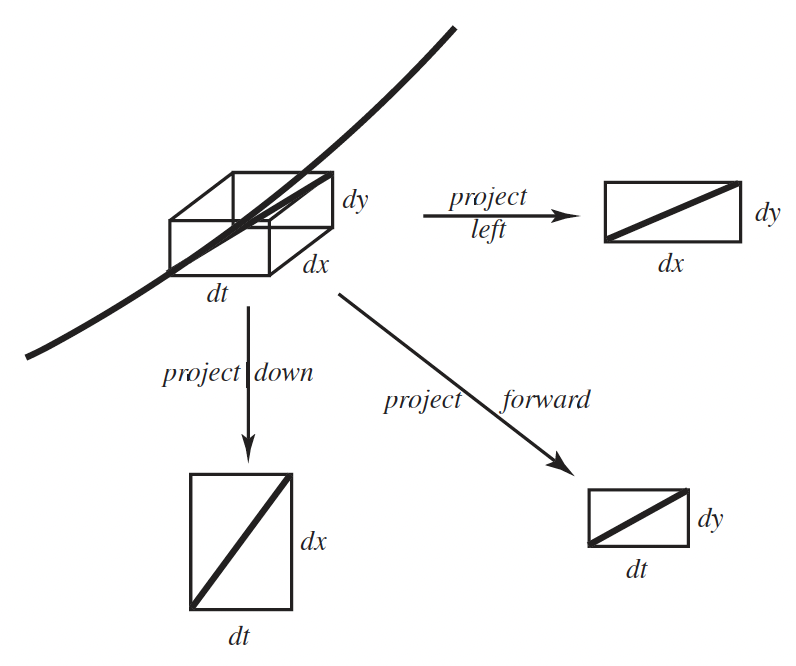
\includegraphics[width=0.6\linewidth]{Figures/Section2/233_parametric_diff.png}
    \caption{We can think of the tangent line as the ratio of the components of the derivatives ${\rm d}x$, ${\rm d}y$, and ${\rm d}t$, and so the relation $\der{y}{x}=\frac{{\rm d}y/{\rm d}t}{{\rm d}x/{\rm d}t}$ follows from simple geometry. (Figure from Tall 2013 ``\textit{How Humans Learn to Think Mathematically}'', Chapter 11).}
    \label{fig:tangent_project}
\end{figure}


The process can be extended to the second derivative (and higher order derivatives). Define
\[
z(t)=\der{y}{x},
\]
then repeat the process to find the derivative of $z$ with respect to $x$:
\[
\der{^2y}{x^2}=\frac{dz}{{\rm d}x}=\frac{dz/{\rm d}t}{{\rm d}x/{\rm d}t}.
\]

Continuing the previous example,
\[
y=\sin t \qquad x=\cos t \qquad \der{y}{x}=-\cot t.
\]
Now
\[
\der{^2y}{x^2}=\frac{dz}{{\rm d}x}=\frac{dz/{\rm d}t}{{\rm d}x/{\rm d}t}
\]
\[
=\frac{d(-\cot t)/{\rm d}t}{-\sin t}=\frac{\csc^2t}{-\sin t}=-\frac{1}{\sin^3t}
\]
\[
=-\frac{1}{y^3}.
\]
Note it is not always convenient to express the derivative in terms of $x$ and $y$.

\newtexpage
\begin{exammistake}
Using
\[
\der{^2y}{x^2}=\frac{d^2y/{\rm d}t^2}{d^2x/{\rm d}t^2}
\]
instead of
\[
\der{^2y}{x^2}=\frac{dz/{\rm d}t}{{\rm d}x/{\rm d}t}, \qquad \text{where} \qquad z=\der{y}{x}.
\]

\begin{quote}
\textbf{25/26 Exam Q2(a)(i).} The equations
\[
x=\sin\left(\frac{\pi t}{6}\right)
\qquad\text{and}\qquad
y=t^2-3t+3
\]
describe a curve in parametric form. Find expressions for ${\rm d}y/{\rm d}x$ and $d^2y/{\rm d}x^2$ in terms of t.
\end{quote}

\textbf{Correct answer:}
\[
\der{^2y}{x^2}
=
\frac{6\left[12\cos\left(\frac{\pi t}{6}\right)+(2t-3)\pi\sin\left(\frac{\pi t}{6}\right)\right]}
{\pi^2\cos^3\left(\frac{\pi t}{6}\right)}. \qquad \checkmark
\]

\textbf{Using the incorrect definition}
\[
\frac{d^2y/{\rm d}t^2}{d^2x/{\rm d}t^2}=-\frac{72}{\pi^2\sin\left(\frac{\pi t}{6}\right)}. \qquad \text{\sffamily X}
\]
\end{exammistake}

\goodbreak
\begin{example}[Lecture]
Find the derivative ${\rm d}y/{\rm d}x$ and the second derivative $d^2y/{\rm d}x^2$ given that
\[
x=t^3+t \qquad y=e^{2t}.
\]
\end{example}
%
\begin{solution}
Find derivatives of $x$ and $y$:
\[
\der{x}{t}=\blank{3t^2+1}
\qquad
\der{y}{t}=\blank{2e^{2t}}.
\]
Take the ratio:
\[
\der{y}{x}=\frac{{\rm d}y/{\rm d}t}{{\rm d}x/{\rm d}t}=\blank{\frac{2e^{2t}}{3t^2+1}}.
\]
Use quotient rule for $dz/{\rm d}t$:
\[
u(t)=\blank{2e^{2t}}
\qquad\text{and}\qquad
v(t)=\blank{3t^2+1}.
\]
Find the derivatives:
\[
u'(t)=\blank{4e^{2t}}
\qquad\text{and}\qquad
v'(t)=\blank{6t}.
\]
Substitute in:
\[
\frac{dz}{{\rm d}t}=\frac{u'v-uv'}{v^2}
=\blank{\frac{4e^{2t}(3t^2+1)-12te^{2t}}{(3t^2+1)^2}}.
\]
and therefore
\[
\der{^2y}{x^2}=\frac{dz/{\rm d}t}{{\rm d}x/{\rm d}t}
=\blank{\frac{4(3t^2-3t+1)}{(3t^2+1)^3}e^{2t}}.
\]
\end{solution}

\begin{recap}{\ref{sec:other_diff_rules}}
    \item \textbf{Implicit differentiation} is performed by differentiating each term in an equation of the form $f(x,y)=0$ with respect to $x$ and rearranging for ${\rm d}y/{\rm d}x$.
    \item \textbf{Logarithmic differentiation} of a function $y=g(x)$ involves taking the log of both sides first to simplify the RHS:
    \[
    \frac{1}{y}\der{y}{x}=\der{}{x}\ln(g(x)).
    \]
    \item To find ${\rm d}y/{\rm d}x$ when $x$ and $y$ are in \textbf{parametric form}, use the relationship
    \[
    \der{y}{x}=\frac{{\rm d}y/{\rm d}t}{{\rm d}x/{\rm d}t}.
    \]
\end{recap}



\end{document}


